%نام و نام خانوادگی:
%شماره دانشجویی: 
\مسئله{LALR یا SLR}
\پاسخ{}
\\
\\
پارسر LALR(1) دقیقا همان استیت‌هایی را تولید می‌کند که SLR(1) تولید می‌کند، فقط چون به lookahead ها به جای followSet توجه می‌کند، conflict های بیش‌تری را می‌تواند در گرامر رفع کند در نتیجه از SLR(1) قوی‌تر است. 
\\
در واقع اگر دقیق‌تر بخواهیم بیان کنیم، اگر به دیاگرام LALR(1) برای یک گرامر نگاه کنیم، می‌توان دید که دقیقا همان استیت‌های SLR(1) را دارد. فقط نکته قابل توجه اینست که اگر در یک استیت باشیم و مثلا به کاراکتر (غیرپایانه) = بربخوریم، اگر در parse table برای SLR(1) به conflict نخوریم و حرکت بعدی ما به طور یکتا مشخص شود، حتما حرکت بعدی ما در LALR(1) هم به طور یکتا مشخص می‌شود، چرا که حروفی که بعد از non-terminal سمت چپ قاعده‌های تولید می‌توانند بیایند، در LALR(1) زیرمجموعه SLR(1) هستند. به عبارتی lookahead های یک non-terminal همیشه زیرمجموعه follow های آن هستند. در نتیجه اگر در SLR(1) تداخلی وجود نداشته باشد، در LALR(1) تداخل نداریم. پس LALR(1) قوی تر از SLR(1) هست.
\\

گرامر زیر که در اسلایدها نیز به آن اشاره شده بود ، با پارسر SLR(1) دارای برخورد است اما با پارسر 
LALR(1)
بدون برخورد پارس می‌شود:
\begin{latin}
\begin{itemize}
    \item 
    S -> E
    \item
    E -> L = R
    \item
    E -> R
    \item
    L -> id
    \item
    L -> *R
    \item
    R -> L
\end{itemize}
\end{latin}
شکل زیر که از اسلایدها برداشته شده است، دیاگرام LALR(1) گرامر بالاست:
\graphicspath{{./images/}}
\begin{center}
	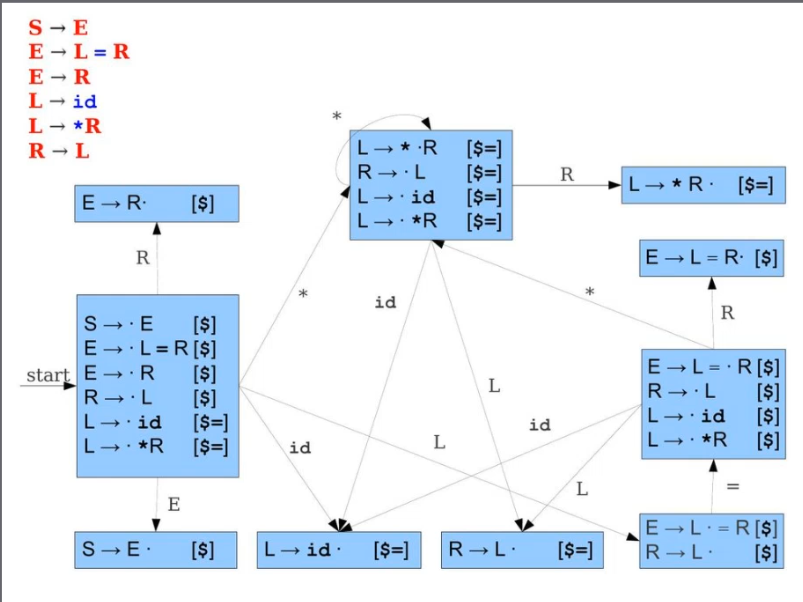
\includegraphics[scale=0.7]{example_diag.png}
\end{center}
در دیاگرام بالا هیچ تداخلی وجود ندارد، اما اگر دیاگرام SLR(1) را برای همین گرامر بکشیم، در استیت پایین سمت راست، تداخل خواهیم داشت. به این صورت که به ازای کاراکتر = هم می‌توان reduce انجام داد و هم می‌توان به استیت بالایی آن shift داد، چون که = جزو follow غیرپایانه R هست پس در SLR(1) می‌توان reduce کرد ولی همان طور که در بالا پیداست، در LALR(1) جزو lookahead برای R نیست پس نمی‌توان reduce کرد. پس مثال مورد نظر پیدا شد.




